%% Neuro-Symbolic Safe Highway Driving — Beamer Presentation
%% Compile: pdflatex presentation.tex  (run twice for cross-refs)
\documentclass[aspectratio=169,10pt]{beamer}

\usetheme{Madrid}
\usecolortheme{seahorse}
\usefonttheme{professionalfonts}

\usepackage{graphicx}
\usepackage{booktabs}
\usepackage{amsmath,amssymb}
\usepackage{xcolor}
\usepackage{tikz}
\usetikzlibrary{arrows.meta,positioning,shapes.geometric,fit,backgrounds}
\usepackage{array}

%% Color palette
\definecolor{neuralblue}{RGB}{31,119,180}
\definecolor{symbolicorange}{RGB}{255,127,14}
\definecolor{nsgreen}{RGB}{44,160,44}
\definecolor{alertred}{RGB}{214,39,40}

%% Enable "visible on=<n->" inside tikzpicture
\tikzset{
  visible on/.style={alt={#1{}{invisible}}},
  invisible/.style={opacity=0},
  alt/.code args={<#1>#2#3}{%
    \alt<#1>{\pgfkeysalso{#2}}{\pgfkeysalso{#3}}%
  },
}

%% Ghost future items instead of hiding them
\setbeamercovered{transparent=15}

\setbeamertemplate{navigation symbols}{}
\setbeamertemplate{footline}[frame number]

\title[Neuro-Symbolic Safe Highway Driving]{%
  \textbf{Neuro-Symbolic Reinforcement Learning}\\
for Safe Autonomous Highway Driving}
\subtitle{LTL-Shielded Deep Q-Networks on HighwayEnv}
\author{Prateek Ganguli}
\date{April 2026}

\begin{document}

% ─────────────────────────────────────────────────────────────────────────────
\begin{frame}
  \titlepage
\end{frame}

% ═════════════════════════════════════════════════════════════════════════════
%  PART 1 — Application, Problem Statement, Success Metric
% ═════════════════════════════════════════════════════════════════════════════

\begin{frame}{Application: Autonomous Highway Driving}
  \begin{columns}[T]
    \begin{column}{0.54\textwidth}
      \textbf{Setting}
      \begin{itemize}[<+->]
        \item 4-lane highway with \textbf{50 surrounding vehicles}
        \item Dense, stochastic traffic: vehicles spawn, merge, and cut in
        \item Ego agent must act in real-time from a partial observation
      \end{itemize}

      \pause\vspace{8pt}
      \textbf{The Core Problem}
      \begin{itemize}[<+->]
        \item \textcolor{neuralblue}{\textbf{Performance:}} drive fast, stay in the rightmost lane
        \item \textcolor{alertred}{\textbf{Safety:}} never collide with another vehicle
        \item \textit{Neural RL ignores safety; pure rules sacrifice performance.}
      \end{itemize}

      \pause\vspace{8pt}
      {\small\textbf{Simulator:} HighwayEnv (Leurent 2018),
      kinematics-based, discrete action space}
    \end{column}
    \begin{column}{0.43\textwidth}
      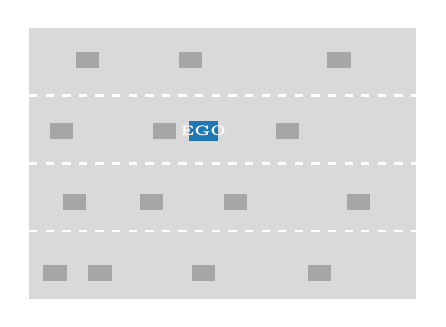
\begin{tikzpicture}[scale=0.82]
        \fill[gray!30] (0,0) rectangle (6,4.2);
        \foreach \y in {1.05,2.1,3.15}{
          \draw[white,dashed,line width=1pt] (0,\y) -- (6,\y);
        }
        \foreach \x/\y in {
          0.4/0.4, 1.1/0.4, 2.7/0.4, 4.5/0.4,
          0.7/1.5, 1.9/1.5, 3.2/1.5, 5.1/1.5,
          0.5/2.6, 2.1/2.6, 4.0/2.6,
        0.9/3.7, 2.5/3.7, 4.8/3.7}{
          \fill[gray!70] (\x-0.18,\y-0.12) rectangle (\x+0.18,\y+0.12);
        }
        \fill[neuralblue] (2.7-0.22,2.6-0.15) rectangle (2.7+0.22,2.6+0.15);
        \node[white,font=\tiny\bfseries] at (2.7,2.6) {EGO};
      \end{tikzpicture}
      \\[4pt]
      {\footnotesize\textit{Ego (blue) navigating dense highway traffic}}
    \end{column}
  \end{columns}
\end{frame}

% ─────────────────────────────────────────────────────────────────────────────
\begin{frame}{Input / Output Specification}
  \begin{columns}[T]
    \begin{column}{0.50\textwidth}
      \textbf{Input: Ego-Relative Observation}\\[4pt]
      \(\mathbf{o}_t \in \mathbb{R}^{10 \times 5}\) (10 nearest vehicles, 5 features each):

      \vspace{5pt}
      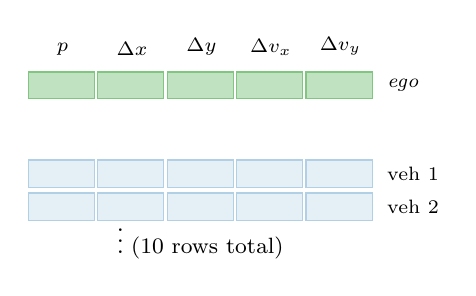
\begin{tikzpicture}[scale=0.84,font=\footnotesize]
        % Column headers
        \foreach \col/\lbl in {0/\(p\), 1/\(\Delta x\), 2/\(\Delta y\), 3/\(\Delta v_x\), 4/\(\Delta v_y\)}{
          \node[anchor=south,font=\scriptsize] at (\col*1.05+0.52,2.35) {\lbl};
        }
        % Ego row (highlighted)
        \foreach \col in {0,...,4}{
          \fill[nsgreen!30,draw=nsgreen!60,line width=0.4pt]
          (\col*1.05,1.85) rectangle (\col*1.05+1.0,2.25);
        }
        \node[font=\scriptsize,right] at (5.28,2.05) {\textit{ego}};
        % Other vehicle rows
        \foreach \row in {0,1}{
          \foreach \col in {0,...,4}{
            \fill[neuralblue!12,draw=neuralblue!35,line width=0.4pt]
            (\col*1.05,\row*0.5) rectangle (\col*1.05+1.0,\row*0.5+0.42);
          }
        }
        \node[font=\scriptsize,right] at (5.28,0.71) {veh 1};
        \node[font=\scriptsize,right] at (5.28,0.21) {veh 2};
        \node[font=\small] at (2.60,-0.22) {\(\vdots\)\;\footnotesize(10 rows total)};
      \end{tikzpicture}

      \vspace{4pt}
      \begin{itemize}\footnotesize
        \item<2-> \(\Delta x,\Delta y\in[-100,100]\) m;\; \(\Delta v\in[-30,30]\) m/s (normalized)
        \item<3-> Sorted by longitudinal distance; rear vehicles included
        \item<4-> Row order shifts each step, making the raw input \textbf{permutation-variant}
      \end{itemize}
    \end{column}
    \begin{column}{0.48\textwidth}
      \onslide<5->{
        \textbf{Output: 5 Discrete Actions}\\[5pt]
        \footnotesize
        \begin{tabular}{cl}
          \toprule
          ID & Action \\\midrule
          0 & \textsc{lane\_left} \\
          1 & \textsc{idle} \\
          2 & \textsc{lane\_right} \\
          3 & \textsc{faster} \\
          4 & \textsc{slower} \\\bottomrule
        \end{tabular}
      }

      \vspace{10pt}
      \onslide<6->{
        \normalsize\textbf{Reward Function}\\[4pt]
        \[
          r_t = \underbrace{0.4\,r_\text{speed}}_{\text{go fast}}
          + \underbrace{0.1\,r_\text{lane}}_{\text{stay right}}
          - \underbrace{\mathbf{1}_\text{crash}}_{\text{survive}}
        \]
        {\footnotesize \(r_\text{speed}\in[0,1]\) linearly from 20 to 30 m/s;
        crash ends the episode.}
      }
    \end{column}
  \end{columns}
\end{frame}

% ─────────────────────────────────────────────────────────────────────────────
\begin{frame}{Success Metrics \& Formal Safety Specification}
  \begin{columns}[T]
    \begin{column}{0.44\textwidth}
      \begin{block}{What counts as success?}
        \textit{100 independent test episodes:}
        \begin{itemize}[<2->]\small
          \item \(\uparrow\) Mean reward (did the agent drive well?)
          \item \(\downarrow\) Crash rate (did it stay safe?)
          \item \(\downarrow\) Reward std (is the behavior consistent?)
        \end{itemize}
      \end{block}
    \end{column}
    \begin{column}{0.54\textwidth}
      \pause
      \begin{alertblock}{Formal Safety Specification (LTL)}
        Four constraints, all enforced \textit{at every timestep}:
        \begin{itemize}[<+->]\small
          \item \textcolor{symbolicorange}{\(\varphi_1\)}: \(\mathbf{G}(\Delta x_\text{front} > 20\text{ m})\) (no tailgating)
          \item \textcolor{symbolicorange}{\(\varphi_2\)}: \(\mathbf{G}(\text{TTC} > 2.0\text{ s})\) (safe time-to-collision)
          \item \textcolor{symbolicorange}{\(\varphi_3\)}: \(\mathbf{G}(\text{LaneLeft} \Rightarrow \neg\text{left\_occ})\)
          \item \textcolor{symbolicorange}{\(\varphi_4\)}: \(\mathbf{G}(\text{LaneRight} \Rightarrow \neg\text{right\_occ})\)
        \end{itemize}
      \end{alertblock}
      \pause\vspace{4pt}
      {\small\textit{These become the symbolic component of our solution.}}
    \end{column}
  \end{columns}
\end{frame}

% ═════════════════════════════════════════════════════════════════════════════
%  PART 2 — Solution
% ═════════════════════════════════════════════════════════════════════════════

\begin{frame}{Solution: LTL-Shielded Pearl DQN}
  \begin{center}
    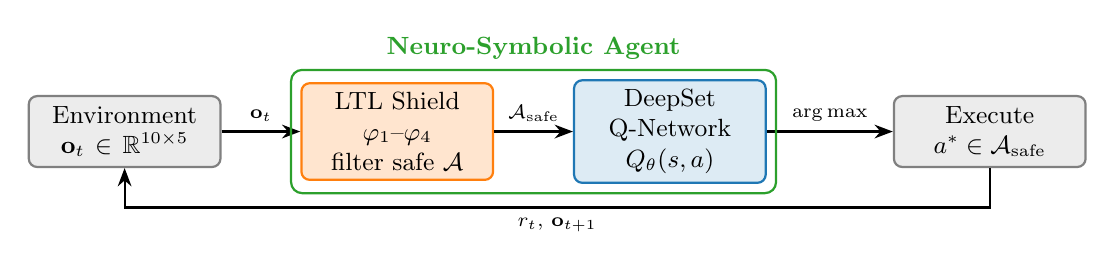
\begin{tikzpicture}[
        box/.style={rectangle,rounded corners=3pt,draw,thick,
        minimum height=0.9cm,text width=2.2cm,align=center,font=\small},
        shield/.style={box,fill=symbolicorange!20,draw=symbolicorange,thick},
        neural/.style={box,fill=neuralblue!15,draw=neuralblue,thick},
        env/.style={box,fill=gray!15,draw=gray,thick},
        arr/.style={-Stealth,thick},
      ]
      \node[env] (obs) {Environment\\\(\mathbf{o}_t \in \mathbb{R}^{10\times5}\)};

      \node[shield,visible on=<2->] (shield) [right=1.0cm of obs]
      {LTL Shield\\\(\varphi_1\text{--}\varphi_4\)\\filter safe \(\mathcal{A}\)};

      \node[neural,visible on=<3->] (dqn) [right=1.0cm of shield]
      {DeepSet\\Q-Network\\\(Q_\theta(s,a)\)};

      \node[env,visible on=<4->] (act) [right=1.6cm of dqn]
      {Execute\\\(a^*\!\in\!\mathcal{A}_\text{safe}\)};

      \draw[arr,visible on=<2->] (obs)    -- (shield)
      node[midway,above,font=\scriptsize]{\(\mathbf{o}_t\)};
      \draw[arr,visible on=<3->] (shield) -- (dqn)
      node[midway,above,font=\scriptsize]{\(\mathcal{A}_\text{safe}\)};
      \draw[arr,visible on=<4->] (dqn)    -- (act)
      node[midway,above,font=\scriptsize]{\(\arg\max\)};
      \draw[arr,visible on=<4->] (act.south) -- ++(0,-0.5) -| (obs.south)
      node[near start,below,font=\scriptsize]{\(r_t,\,\mathbf{o}_{t+1}\)};

      \node[draw=nsgreen,rounded corners,thick,visible on=<3->,
        fit=(shield)(dqn),
        label={[nsgreen,font=\small\bfseries,visible on=<3->]above:%
      Neuro-Symbolic Agent}] {};
    \end{tikzpicture}
  \end{center}

  \vspace{2pt}
  \begin{columns}[T]
    \begin{column}{0.50\textwidth}
      \onslide<5->{%
        \textbf{Key Design Decision}\\[2pt]
        {\small Shield acts \emph{inside} \texttt{env.step()}, not post-hoc.
          Bellman update therefore uses only safe next-state actions:
        \(\;y = r + \gamma\!\max_{a'\in\mathcal{A}_\text{safe}(s')} Q_{\bar\theta}(s',a')\)}
      }
    \end{column}
    \begin{column}{0.48\textwidth}
      \onslide<6->{%
        \textbf{Three Agents Compared}\\[2pt]
        {\small
          \textcolor{neuralblue}{\textbf{Pure Neural}} (Pearl DQN, no constraints)\\[2pt]
          \textcolor{symbolicorange}{\textbf{Pure Symbolic}} (hand-coded FSM, 4 states)\\[2pt]
        \textcolor{nsgreen}{\textbf{Neuro-Symbolic}} (Shielded Pearl DQN)}
      }
    \end{column}
  \end{columns}
\end{frame}

% ─────────────────────────────────────────────────────────────────────────────
\begin{frame}{Neural Component: DeepSet Q-Network}
  \begin{columns}[T]
    \begin{column}{0.50\textwidth}
      \textbf{Why a DeepSet?}\\[4pt]
      Vehicle rows shift each timestep, making the raw input permutation-variant.
      DeepSet aggregation is \textbf{order-invariant by construction}:
      \[
        Q(s,a) = \rho\!\left(\textstyle\sum_{i=1}^{10} \phi(\mathbf{v}_i)\right)
      \]
      \begin{itemize}[<2->]\small
        \item Encoder \(\phi\): shared MLP \([5\!\to\!64\!\to\!64]\) per vehicle
        \item Aggregation: element-wise sum (permutation-invariant)
        \item Head \(\rho\): MLP \([69\!\to\!256\!\to\!256\!\to\!5]\)
      \end{itemize}
    \end{column}
    \begin{column}{0.48\textwidth}
      \pause
      \textbf{Training: Double DQN + PER}
      \begin{itemize}[<+->]\small
        \item Double Q-learning: separate target network reduces overestimation
        \item Prioritized replay (\(\alpha{=}0.6\), \(\beta{:}0.4{\to}1.0\)): focus on high-error transitions
        \item Shield penalty \(-0.05\): incentivizes the policy to internalize safety
      \end{itemize}

      \pause\vspace{6pt}
      {\footnotesize
        \begin{tabular}{@{}ll@{}}
          Buffer  & 15\,000 transitions \\
          LR      & \(5\times10^{-4}\) \\
          \(\gamma\)  & \(0.8\) \\
          \(\varepsilon\) & \(1.0 \to 0.05\) (100k steps) \\
      \end{tabular}}
    \end{column}
  \end{columns}
\end{frame}

% ─────────────────────────────────────────────────────────────────────────────
\begin{frame}{Symbolic Component: LTL Safety Shield}
  \begin{columns}[T]
    \begin{column}{0.50\textwidth}
      \textbf{Four Globally-Enforced Predicates}
      \begin{itemize}[<+->]\small
        \item \textcolor{symbolicorange}{\(\varphi_1\)}: No tailgating (\(\Delta x_\text{front} > 20\) m)
        \item \textcolor{symbolicorange}{\(\varphi_2\)}: Safe TTC (\(> 2.0\) s)
        \item \textcolor{symbolicorange}{\(\varphi_3\)}: Lane-left only if left lane is clear
        \item \textcolor{symbolicorange}{\(\varphi_4\)}: Lane-right only if right lane is clear
      \end{itemize}

      \pause\vspace{6pt}
      \textbf{Shield Evaluation (per step)}
      \begin{enumerate}[<+->]\small
        \item Decode \(\mathbf{o}_t\) into per-vehicle predicates
        \item For each candidate action, simulate one step symbolically
        \item Retain \(a\) iff \(\varphi_1\wedge\varphi_2\wedge\varphi_3\wedge\varphi_4\) holds
        \item Return \(\mathcal{A}_\text{safe}\subseteq\{0,\ldots,4\}\) to Q-network
      \end{enumerate}
    \end{column}
    \begin{column}{0.48\textwidth}
      \pause
      \textbf{Implementation}\\[4pt]
      Built on \textbf{Meta's Pearl} framework.
      \texttt{LTLShieldSafetyModule} implements Pearl's \texttt{SafetyModule} ABC, making it modular and composable.

      \vspace{10pt}
      \pause
      \textbf{What this guarantees}
      \begin{itemize}[<+->]\small
        \item Every approved action satisfies \(\varphi_1\)--\(\varphi_4\) by construction
        \item Each veto is \textbf{human-readable}: \textit{``\(\varphi_3\) violated: left lane occupied''}
        \item No gradient computation; purely symbolic evaluation
      \end{itemize}
    \end{column}
  \end{columns}
\end{frame}

% ═════════════════════════════════════════════════════════════════════════════
%  PART 3 — Neuro-Symbolic Checklist
% ═════════════════════════════════════════════════════════════════════════════

\begin{frame}{Neuro-Symbolic Checklist: The Two Parts}
  \begin{columns}[T]
    \begin{column}{0.48\textwidth}
      \begin{block}{1.\ The Neuro Part}
        \textcolor{neuralblue}{\textbf{DeepSet Double-DQN with PER}}
        \begin{itemize}[<2->]\small
          \item Learns a Q-function from raw interactions (100k steps)
          \item Discovers \emph{when} to speed up, slow down, or change lane
          \item DeepSet encoder generalizes across any vehicle ordering
          \item Policy learns to respect the shield: override rate falls during training
        \end{itemize}
      \end{block}
    \end{column}
    \begin{column}{0.50\textwidth}
      \pause
      \begin{block}{2.\ The Symbolic Part}
        \textcolor{symbolicorange}{\textbf{LTL Safety Shield}} (\(\varphi_1\)--\(\varphi_4\))
        \begin{itemize}[<+->]\small
          \item Encodes expert safety knowledge as inviolable logical rules
          \item Deterministic predicate evaluation; no training required
          \item Provides a \textbf{hard filter} on the Q-network's action choices
          \item If the shield approves \(a\), no known unsafe outcome follows
        \end{itemize}
      \end{block}
    \end{column}
  \end{columns}
\end{frame}

% ─────────────────────────────────────────────────────────────────────────────
\begin{frame}{Neuro-Symbolic Checklist: Generalization \& Fragility}
  \begin{columns}[T]
    \begin{column}{0.48\textwidth}
      \begin{block}{3.\ Generalization of the Neuro Part}
        \begin{itemize}[<2->]\small
          \item Permutation invariance: \(\sum_i\phi(\mathbf{v}_i)\) is independent of vehicle ordering, handling any traffic configuration
          \item Reward varies continuously with speed, giving the network a smooth training signal
          \item Limitation: does not transfer to unseen action spaces or sensor modalities
        \end{itemize}
      \end{block}
    \end{column}
    \begin{column}{0.50\textwidth}
      \pause
      \begin{alertblock}{4.\ Fragility of the Symbolic Part}
        \begin{itemize}[<+->]\small
          \item Coverage gaps: \(\varphi_1\)--\(\varphi_4\) miss diagonal or merging-at-speed scenarios
          \item Sensor noise: noisy kinematics can flip predicate truth values
          \item Fixed thresholds: 20 m gap, 2 s TTC, conservative and not adaptive
          \item Spawn crashes: vehicles appearing adjacent bypass the 1-step lookahead
        \end{itemize}
      \end{alertblock}
    \end{column}
  \end{columns}
\end{frame}

% ─────────────────────────────────────────────────────────────────────────────
\begin{frame}{Neuro-Symbolic Checklist: Benefits}
  \textbf{5.\ Benefits of the Combination}

  \vspace{8pt}
  \begin{columns}[T]
    \begin{column}{0.32\textwidth}
      \onslide<2->{
        \begin{exampleblock}{Safety \& Explainability}
          \small
          Crash rate:\\[2pt]
          \textbf{27\%\;\(\to\)\;18\%}\\[4pt]
          Each shield veto has a human-readable reason (\(\varphi_i\) violated)
        \end{exampleblock}
      }
    \end{column}
    \begin{column}{0.32\textwidth}
      \onslide<3->{
        \begin{exampleblock}{Consistency}
          \small
          Reward std:\\[2pt]
          \textbf{16.3\;\(\to\)\;11.4}\;(\({-}30\%\))\\[4pt]
          Shield prevents catastrophic exploratory crashes early in training
        \end{exampleblock}
      }
    \end{column}
    \begin{column}{0.32\textwidth}
      \onslide<4->{
        \begin{exampleblock}{Data Efficiency}
          \small
          Smaller safe action space yields cleaner, faster exploration\\[4pt]
          Override penalty steers the reward signal toward safe behavior
        \end{exampleblock}
      }
    \end{column}
  \end{columns}

  \vspace{8pt}
  \onslide<5->{
    \begin{block}{\centering Combined Effect}
      \centering\small
      After controlling for spawn crashes: FSM = 23.5\%, Neural = 23.2\%; \emph{neither alone beats the other.}\\
      Neuro-Symbolic achieves \textbf{18.0\%}: the gain exceeds what either component produces alone.
    \end{block}
  }
\end{frame}

% ═════════════════════════════════════════════════════════════════════════════
%  PART 4 — Results
% ═════════════════════════════════════════════════════════════════════════════

\begin{frame}{Results: Training Dynamics}
  \begin{columns}[T]
    \begin{column}{0.50\textwidth}
      \begin{figure}
        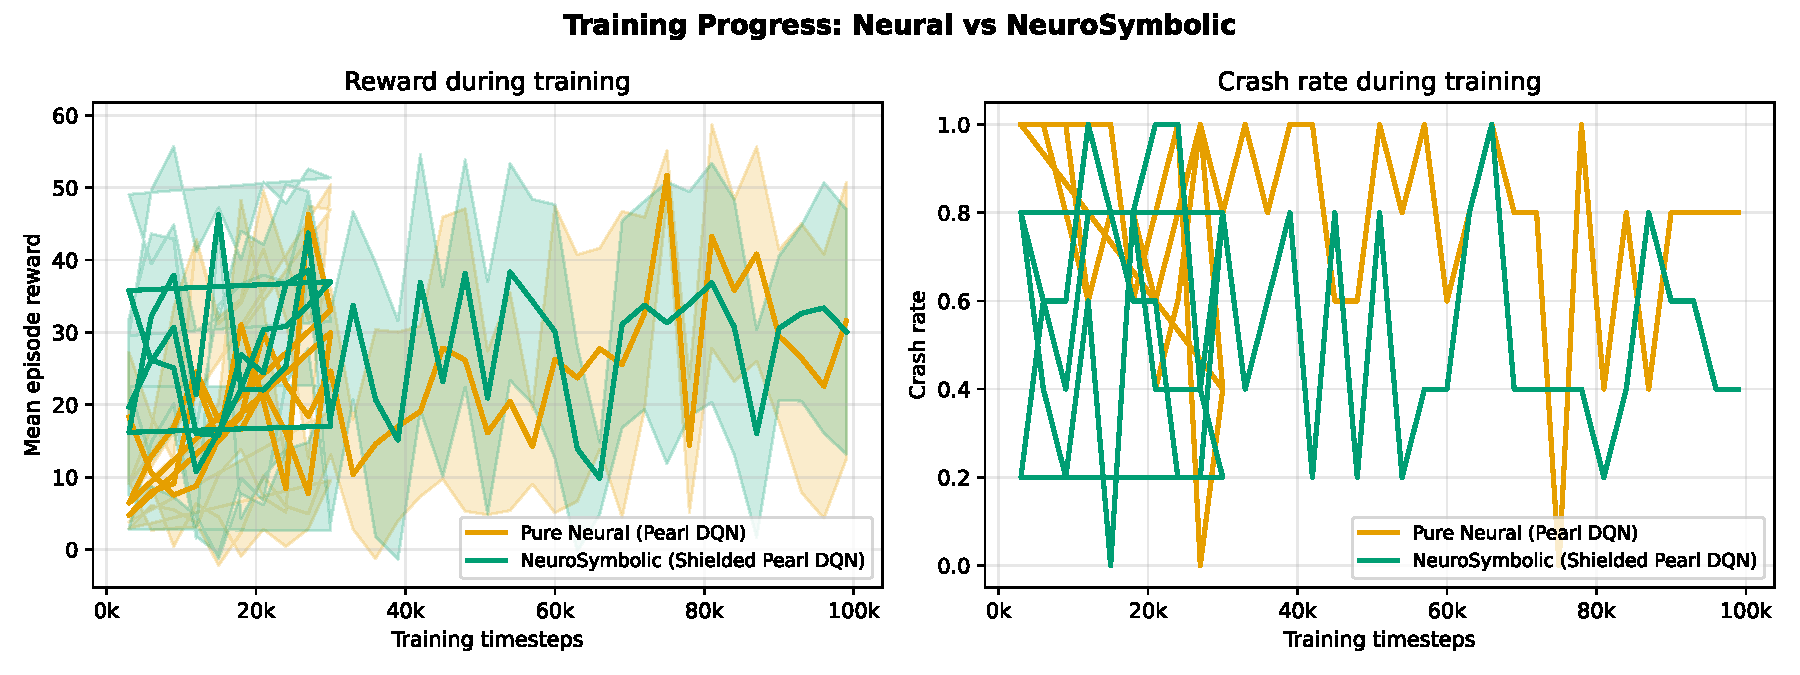
\includegraphics[width=\linewidth]{fig1_training_curves.pdf}
        \caption{\small Training reward \& crash rate vs.\ timestep (100k steps)}
      \end{figure}
    \end{column}
    \begin{column}{0.48\textwidth}
      \begin{figure}
        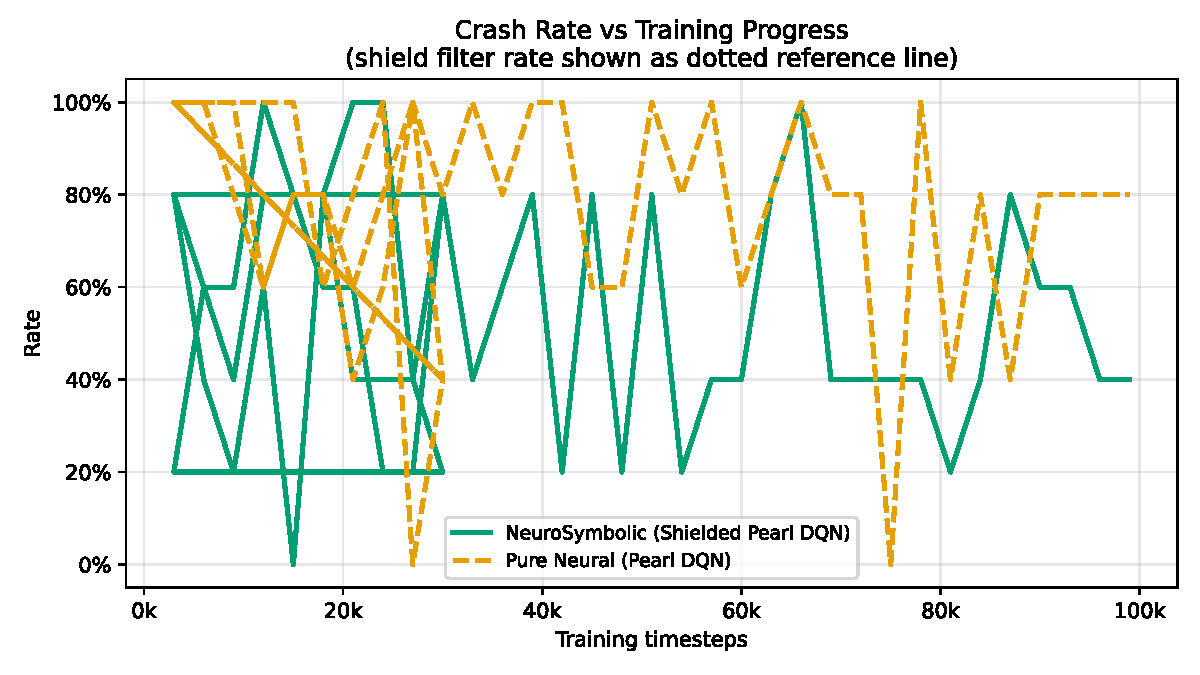
\includegraphics[width=\linewidth]{fig3_shield_filter.pdf}
        \caption{\small Shield override rate during training}
      \end{figure}
    \end{column}
  \end{columns}

  \pause\vspace{2pt}
  \begin{itemize}[<+->]\small
    \item \textbf{Neural} reward rises faster, but unconstrained exploration yields more crashes
    \item Shield \textbf{override rate decreases} over training: policy learns to avoid vetoes
    \item Shielded agent reaches a \textbf{lower steady-state crash rate} despite slower initial reward growth
  \end{itemize}
\end{frame}

% ─────────────────────────────────────────────────────────────────────────────
\begin{frame}{Results: 100-Episode Evaluation}
  \begin{columns}[T]
    \begin{column}{0.50\textwidth}
      \begin{figure}
        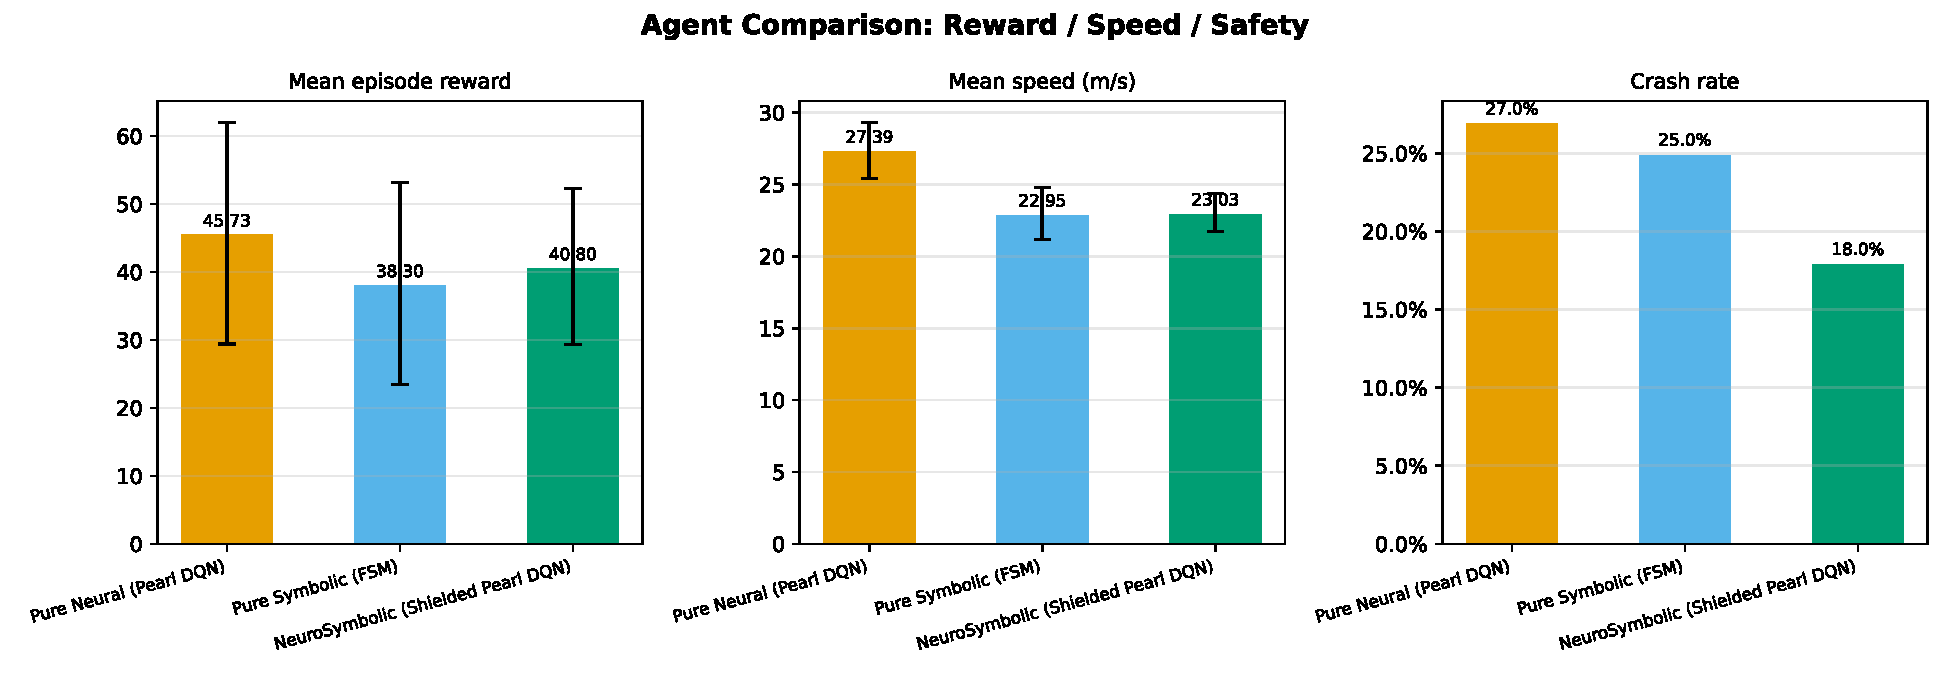
\includegraphics[width=\linewidth]{fig2_bar_comparison.pdf}
        \caption{\small Reward / speed / crash rate comparison}
      \end{figure}
    \end{column}
    \begin{column}{0.48\textwidth}
      \begin{figure}
        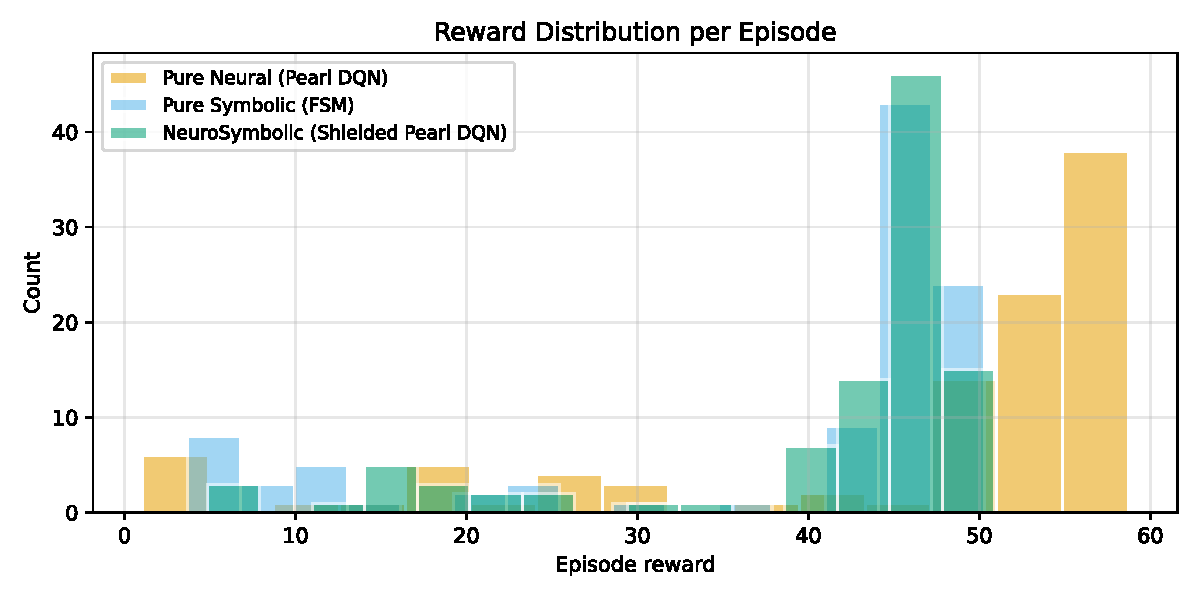
\includegraphics[width=\linewidth]{fig4_reward_distribution.pdf}
        \caption{\small Reward distribution across 100 episodes}
      \end{figure}
    \end{column}
  \end{columns}

  \pause
  \begin{center}\small
    \begin{tabular}{lrrrr}
      \toprule
      Agent & Reward\;\(\uparrow\) & Speed\;\(\uparrow\) & Crash\;\(\downarrow\) & Std\;\(\downarrow\) \\\midrule
      \textcolor{neuralblue}{Pure Neural}           & 45.7 & 27.4\,m/s & 27\% & 16.3 \\
      \textcolor{symbolicorange}{Pure Symbolic (FSM)} & 38.3 & 23.0\,m/s & 25\% & 14.8 \\
      \textcolor{nsgreen}{\textbf{Neuro-Symbolic}}  & \textbf{40.8} & 23.0\,m/s & \textbf{18\%} & \textbf{11.4} \\
      \bottomrule
    \end{tabular}
  \end{center}
\end{frame}

% ─────────────────────────────────────────────────────────────────────────────
\begin{frame}{Results: Controlling for Spawn-Induced Crashes}
  \begin{columns}[T]
    \begin{column}{0.50\textwidth}
      \begin{figure}
        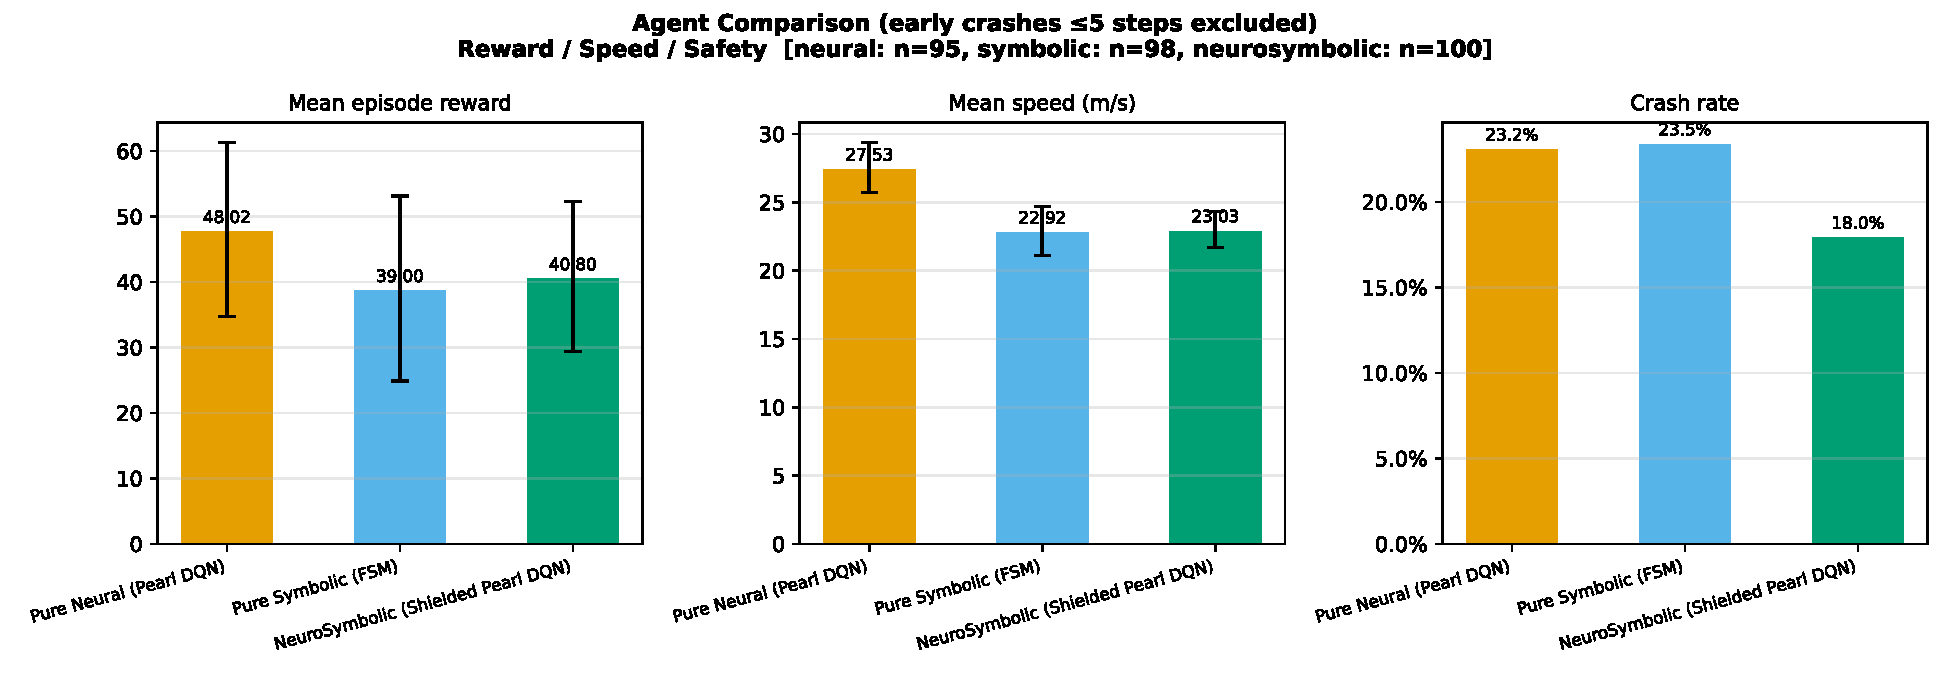
\includegraphics[width=\linewidth]{fig5_bar_comparison_filtered.pdf}
        \caption{\small Episodes with crash in \(\leq 5\) steps removed}
      \end{figure}
    \end{column}
    \begin{column}{0.48\textwidth}
      \textbf{Why filter?}
      \begin{itemize}\small
        \item HighwayEnv can spawn vehicles directly adjacent to ego
        \item Crash \(\leq\)5 steps: \emph{environment artifact}, not policy failure
        \item Filtering isolates \emph{policy-attributable} crashes
      \end{itemize}

      \pause
      \small
      \begin{tabular}{lrr}
        \toprule
        Agent & \(n\) & Crash Rate\\\midrule
        \textcolor{neuralblue}{Neural}                        & 95  & 23.2\%\\
        \textcolor{symbolicorange}{Symbolic}                  & 98  & 23.5\%\\
        \textcolor{nsgreen}{\textbf{Neuro-Sym.}} & \textbf{100} & \textbf{18.0\%}\\
        \bottomrule
      \end{tabular}

      \pause\vspace{-1pt}
      \begin{itemize}[<+->]\small
        \item Only Neuro-Sym.\ has \textbf{zero} spawn crashes; the shield blocks proximity collisions too
        \item FSM \emph{equals} neural after filtering; pure rules add nothing without learning
        \item \textbf{5.2 pp} gap: attributable to the combined policy-shield effect
      \end{itemize}
    \end{column}
  \end{columns}
\end{frame}

% ─────────────────────────────────────────────────────────────────────────────
\begin{frame}{Discussion \& Conclusions}
  \begin{columns}[T]
    \begin{column}{0.48\textwidth}
      \textbf{What Worked}
      \begin{itemize}[<2->]\small
        \item Environment-level shielding ensures correct Bellman targets
        \item DeepSet handles permutation variance; policy focuses on strategy
        \item Override penalty measurably incentivizes safety internalization
        \item Best safety-consistency trade-off across all three agents
      \end{itemize}
    \end{column}
    \begin{column}{0.50\textwidth}
      \pause
      \textbf{Limitations \& Future Work}
      \begin{itemize}[<+->]\small
        \item Reward gap: \(\sim\)5 pts lost to conservative shielding; adaptive thresholds could close this
        \item Spawn crashes: need multi-step lookahead or a probabilistic shield
        \item Learned specs: neural-guided LTL synthesis is an open direction
        \item Scaling: continuous action spaces require differentiable shields
      \end{itemize}
    \end{column}
  \end{columns}

  \pause\vspace{8pt}
  \begin{block}{\centering Bottom Line}
    \centering
    Combining a \textcolor{neuralblue}{\textbf{learned DeepSet Q-network}} with a
    \textcolor{symbolicorange}{\textbf{formal LTL safety shield}}\\[2pt]
    reduces crash rate by \textbf{33\%} and reward variance by \textbf{30\%}
    versus pure neural; each blocked action is traceable to a named rule.
  \end{block}
\end{frame}

\end{document}
